%%%%%%%%%%%%%%%%%%%%%%%%%%%%%%%%%%%%%%%%%%%%%%%%%%%%%%%%%%%%%%%%%%%%%%%%
\chapter{Motivation}
%%%%%%%%%%%%%%%%%%%%%%%%%%%%%%%%%%%%%%%%%%%%%%%%%%%%%%%%%%%%%%%%%%%%%%%%

\begin{figure}[ht]
    \centering
    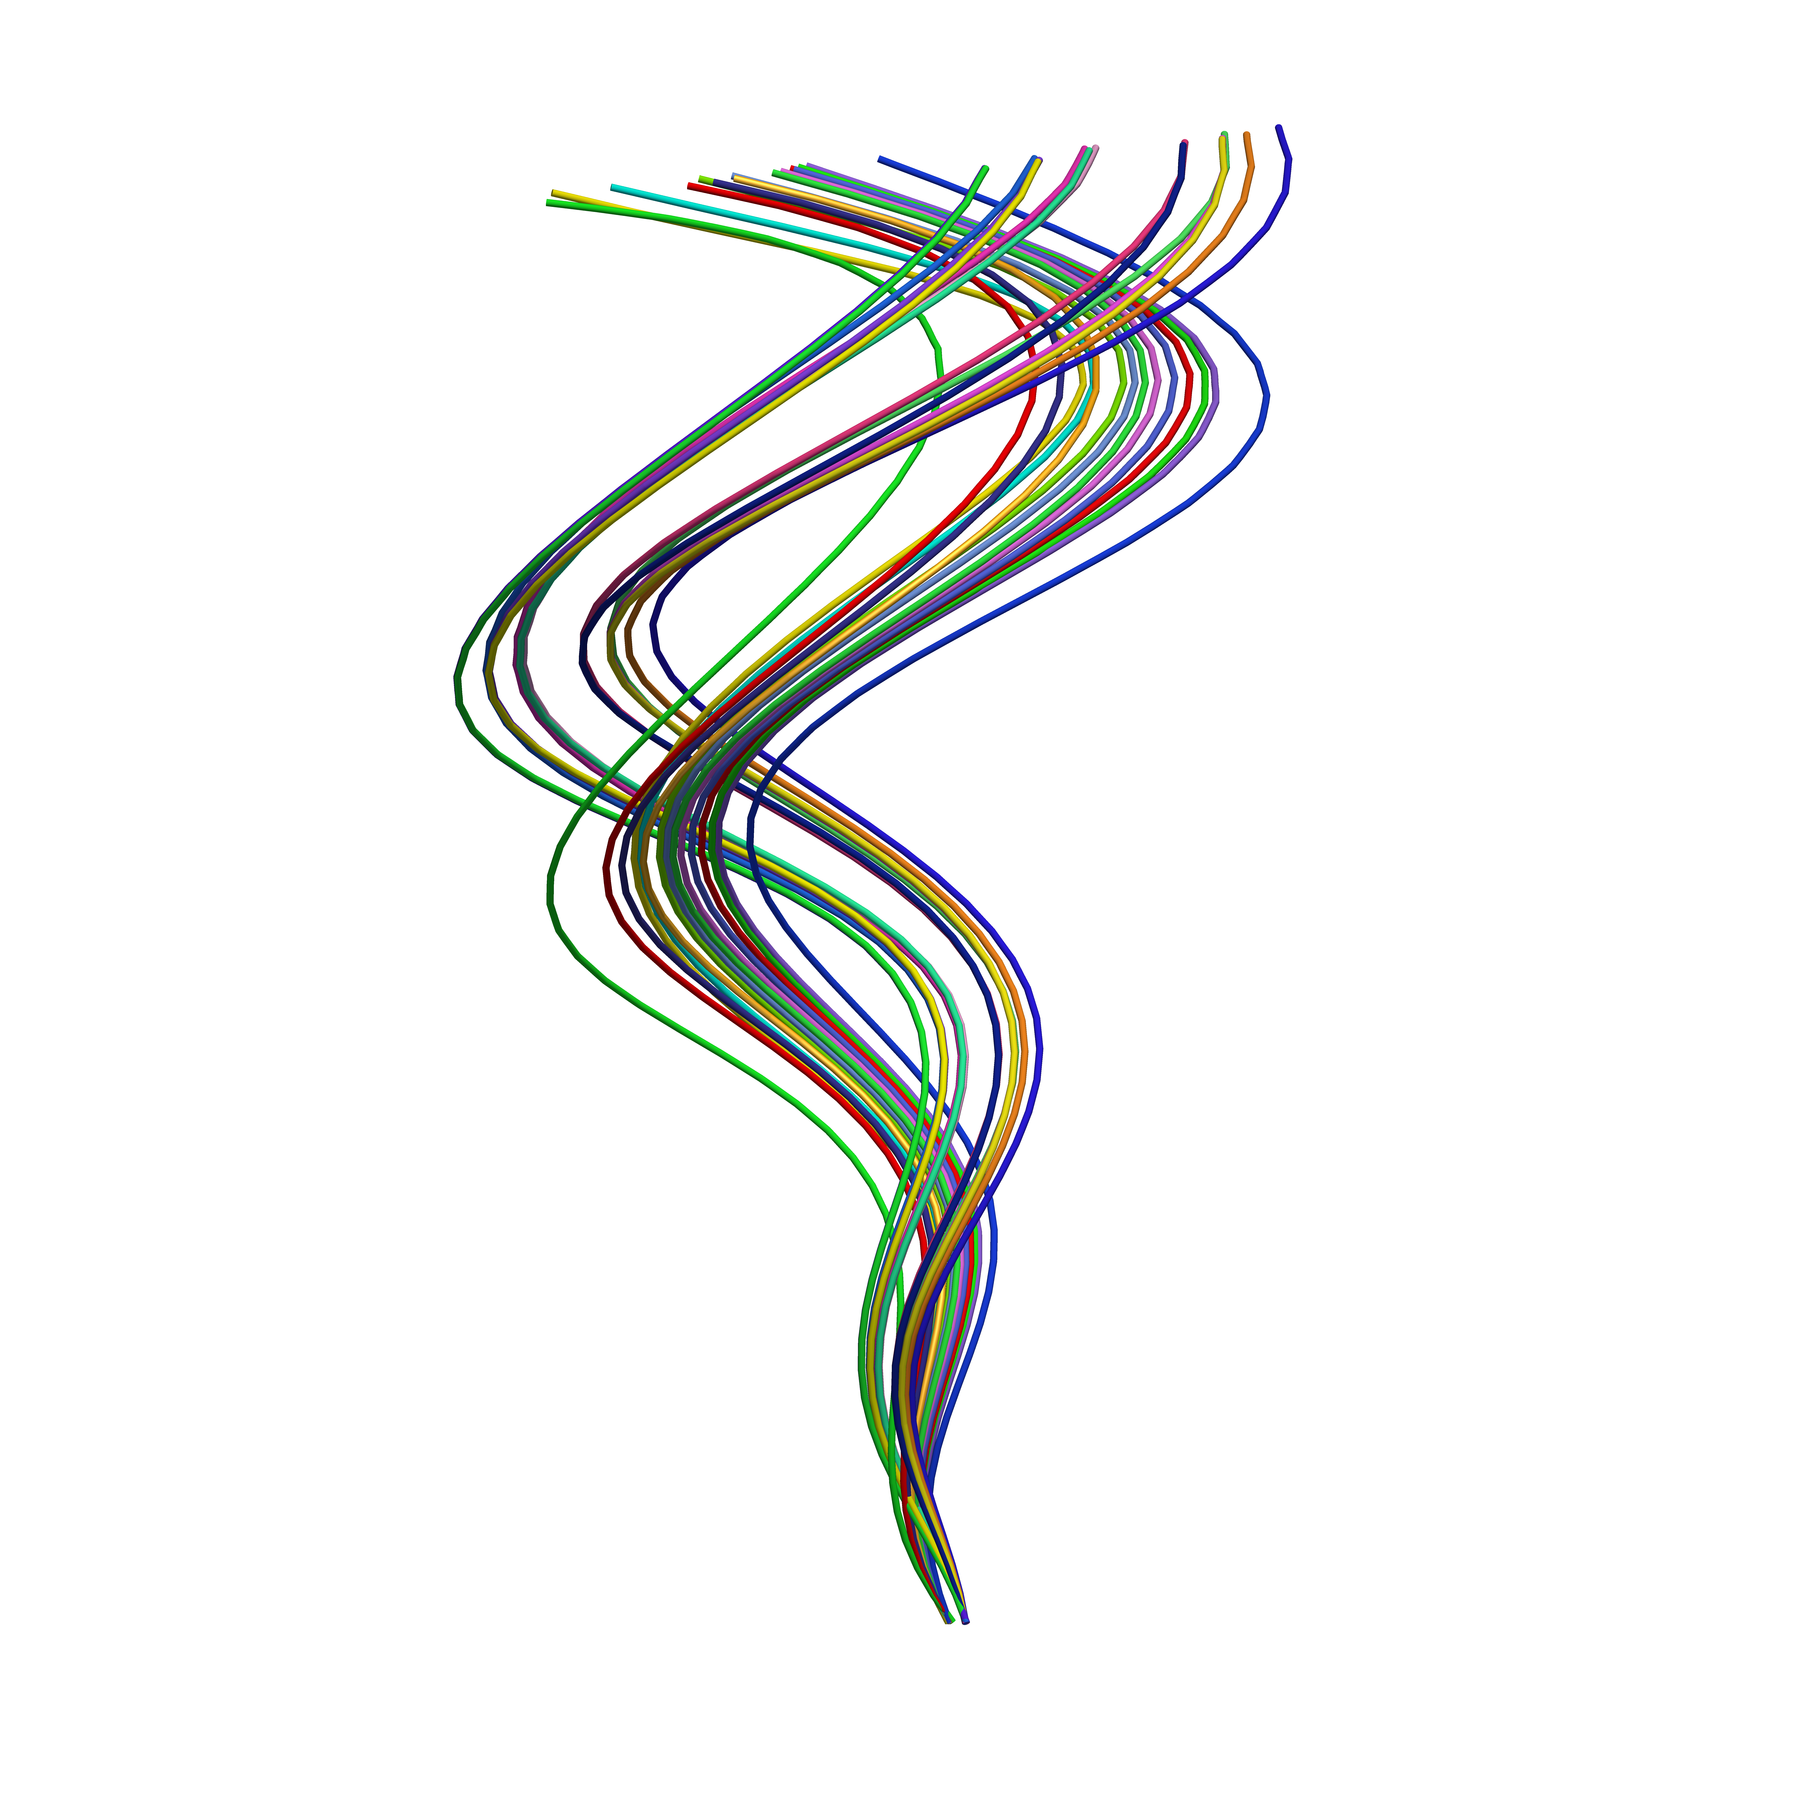
\includegraphics[width=0.75\textwidth]{Images/vcores.png}
    \caption{Spaghetti plot of 30 vortex core lines from a set of flow
    fields. The lines have a similar origin at the bottom of the image,
    but then deviate upwards with increasing differences. The quantity
    of the variance is not easily determined, as overlapping lines are
    not distinguishable.}
    \label{fig:spaghetti}
\end{figure}
The graphical depiction of uncertainty has for a long time been a field
of visualization, which has not been receiving a lot of attention. But,
with todays available computing power, not only the amount of data
increased, but also the ways in which the data can be aquired. With data
more often coming from simuilations or multiple calculations with
varying parameters, the visualization of uncertainty is of rising
importance. Multiple flows through the same system used to be modeled
with spaghetti plots, yielding a line for each member. Figure
\ref{fig:spaghetti} shows a spaghetti plot of the vortex core lines of
members of an uncertain vector domain. A vortex is a region in which the
flow revolves around a line, the core line. The vortices of these fields
all start at a similar position and then twist upwards with varying
radii and acceleration. The problem with this approach is, that the
united parts are hard to distinguish, unallowing for a decision about
the quantity of uncertainty at a location. With increasing member size,
the image becomes cluttered, but high frequency areas are not
necessarily easy to see and the visualization can not be considered
accurate without indications for error, accuracy of confidence.\\
\indent This was until 2012 Mathias Otto und Holger Theisel presented
their approach for extracting probabilities for the existence of a
vortex core line in a cell. They were the first to expand the
multivariate Gaussian sampling to a neighborhood of a vector field,
giving them normally distributed derivatives. This allowed them to
process their sampled cells using the Parallel Vectors operator, to find
the points at which the velocity vector is parallel to its derived
acceleration vector. If now the Jacobian matrix at the found point has a
pair of complex conjugate eigenvalues, the point lies on a vortex.
Complex eigenvalues denote a rotational transformation. The relative
number of positive samples are then the probability for a vortex core
line in that cell. Figure~\ref{fig:UVC} shows the result of the
uncertain vortex calculation for the whole set of vector fields from
Figure~\ref{fig:spaghetti}. The set is very uncertain. As the vortices
all have a similar base and start to deviate upwards, there are red
region with high probability at the bottom. From there on up, the lines
spread and therefore there are wider regions with low probability. This
directly highlights common regions of the individual members and eases
the understanding of the uncertainty in the fields.\\
\indent As the derivative of a scalar field is a vector field, an idea
that comes to mind is to apply their method to the extraction of
features from uncertain scalar fields. For the extraction of a ridge
line from an 3-dimensional scalar field, the approach is basically the
same. We only require an extra step, calculating the gradient of the
sampled scalar field, to get an uncertain vector field in which we can
search for similar criteria. The Parallel Vectors operator is easily
adjusted to give the points where the gradient is parallel to its major
eigenvector and the eigenvalues of the Hessian, the counterpart to the
Jacobian, don't need to be complex, but negative. The extraction of a
ridge surfaces on the other hand is a bit different as we are searching
for orthogonality of the gradient and the minor eigenvector. An adjusted
variant of the Marching Cubes algorithm would give us an approximation
of the uncertain ridge surface, but this method has some problems,
especially at volatile locations of the fields, where the ridge of the
individual members is already weak. The next chapter will give detailed
information on the problems coming with Uncertain Marching Cubes and how
we tried to overcome them.

\begin{figure}[t]
    \centering
    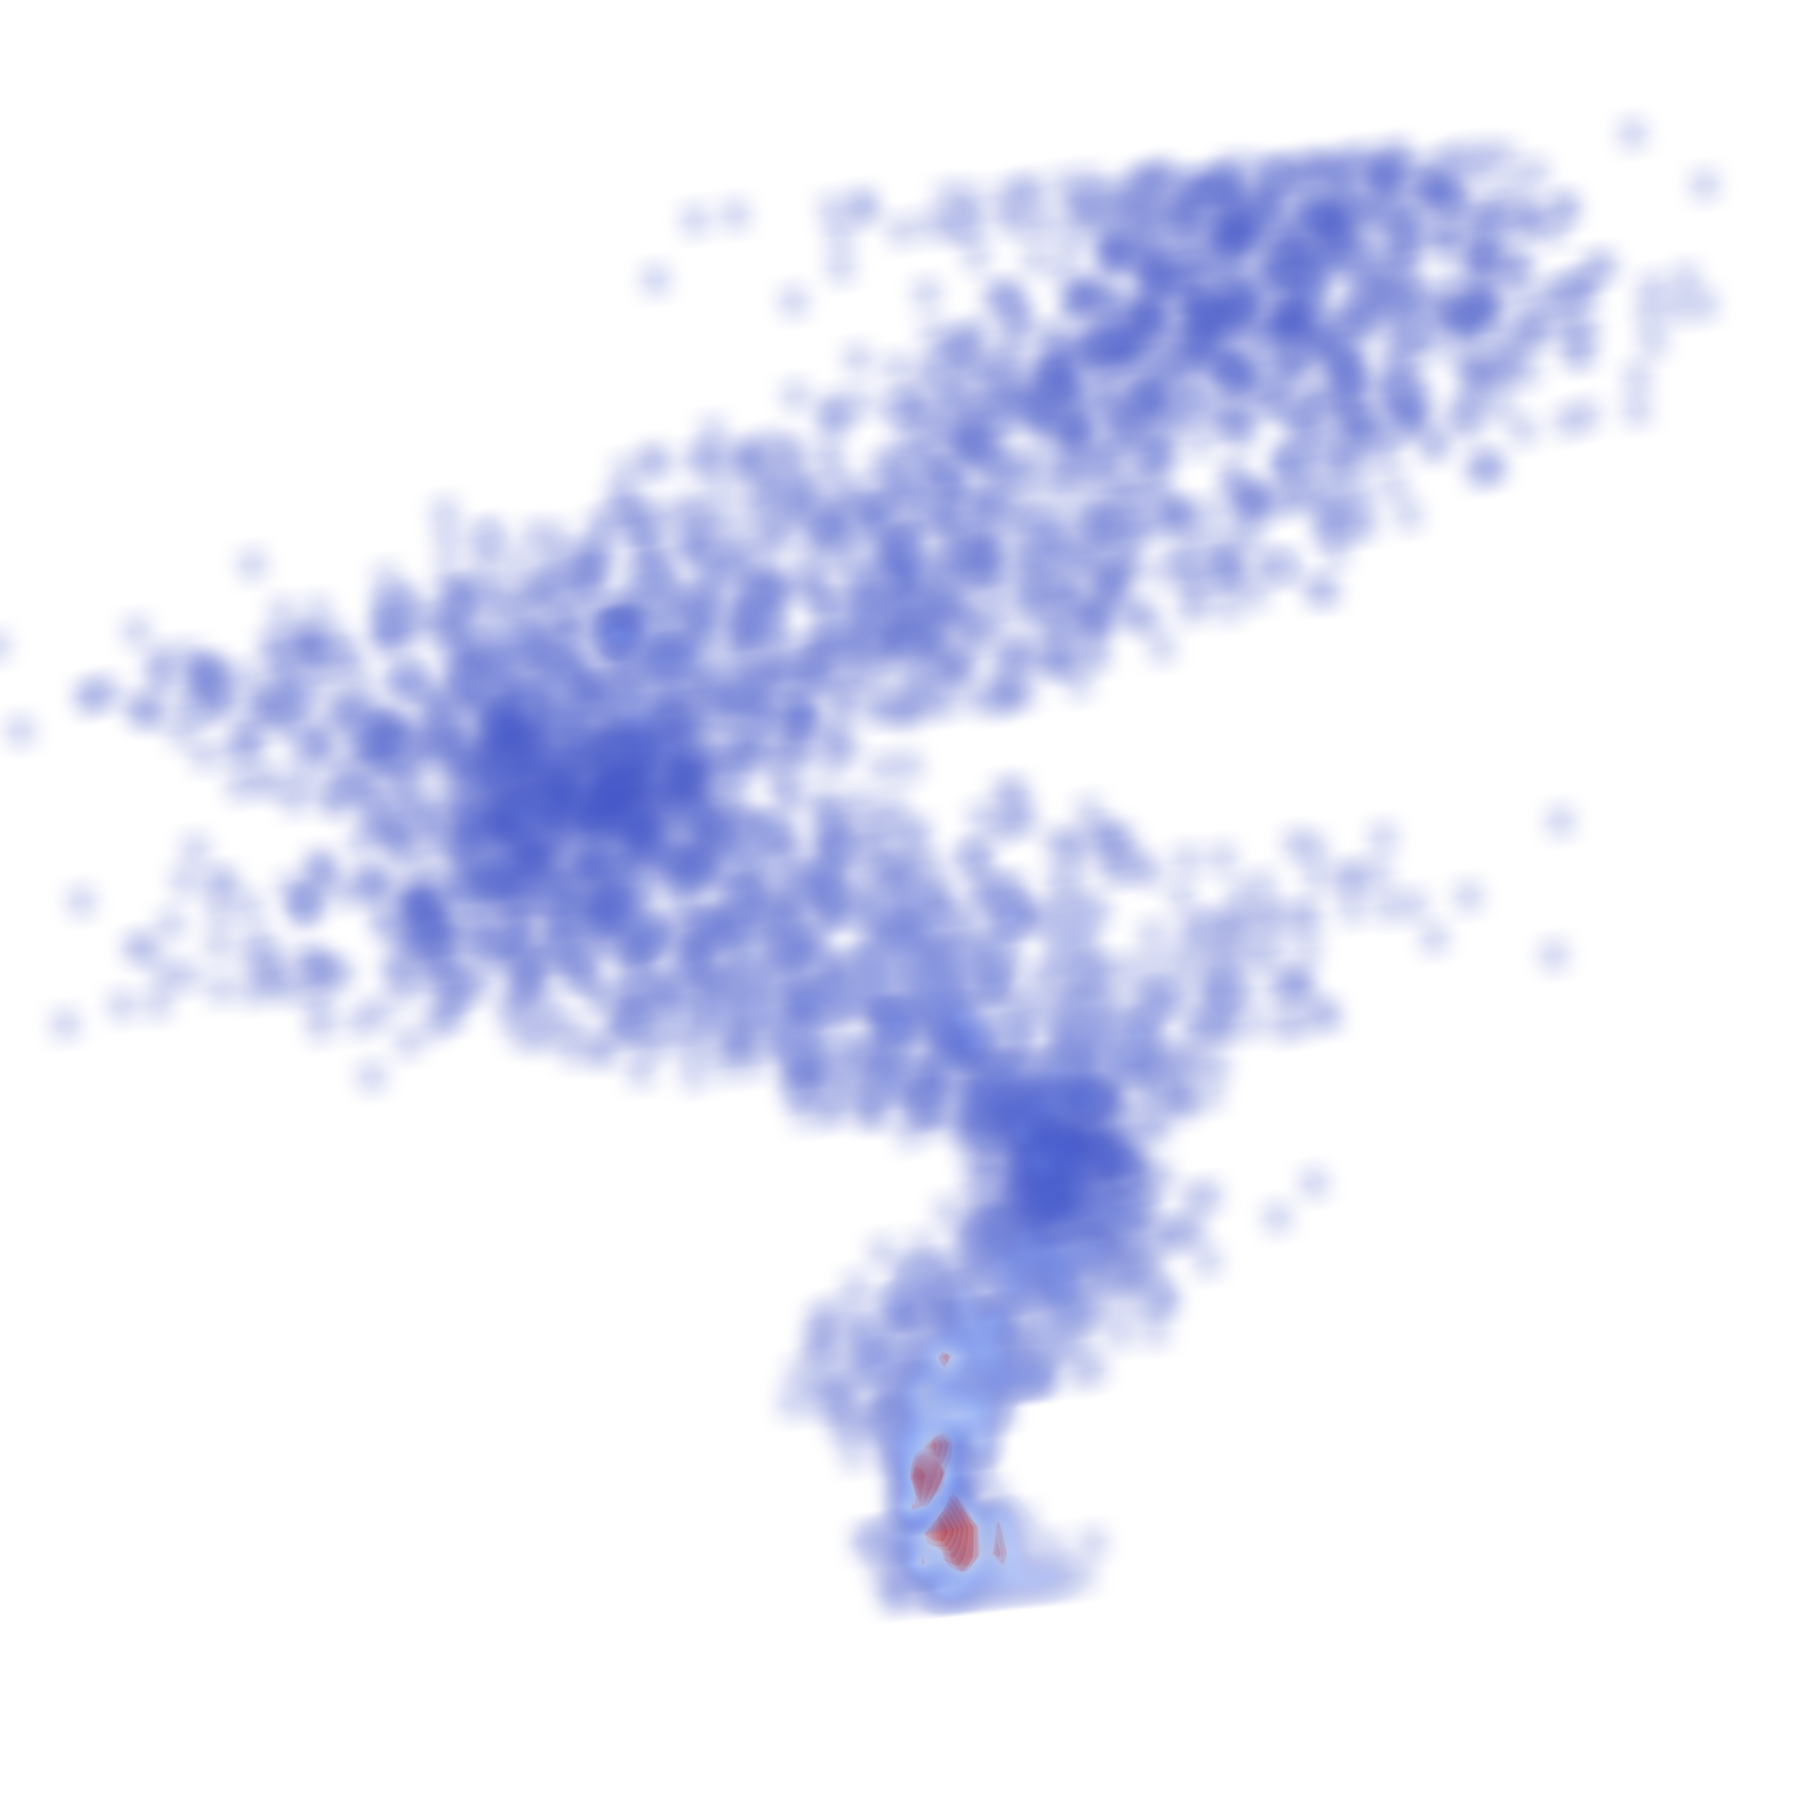
\includegraphics[width=0.75\textwidth]{Images/unccores.png}
    \caption{Uncertain vortex core lines for the full set of correlated
    flow fields. Region with probability reaching $100\%$ at the bottom,
    where the core lines originate. The individual lines originate from
    minor changes of the general direction and radius. As the line expands
    upwards, these changes become more and more visible, leading to an
    increasind spread of the uncertain visualization.}
    \label{fig:UVC}
\end{figure}